% Modelo conceitual (MER, notacao de Chen). Gera MERConceitual.png.
\documentclass[border=8pt]{standalone}
\usepackage[utf8]{inputenc}
\usepackage[T1]{fontenc}
\usepackage{tikz}
\usetikzlibrary{shapes.geometric,positioning,calc}
\definecolor{azul}{RGB}{24,90,160}
\definecolor{azulclaro}{RGB}{230,240,250}
\definecolor{marrom}{RGB}{130,82,14}
\definecolor{bege}{RGB}{250,238,220}
\tikzset{
  ent/.style={rectangle, rounded corners=6pt, draw=azul, fill=azulclaro, line width=0.7pt,
    minimum height=0.9cm, minimum width=2.4cm, inner xsep=8pt, font=\sffamily\large, text=azul!80!black},
  rel/.style={diamond, aspect=2.4, draw=marrom, fill=bege, line width=0.7pt, inner sep=1pt,
    font=\sffamily, text=marrom!60!black},
  lig/.style={draw=black!60, line width=0.6pt},
  card/.style={font=\sffamily\small, text=black!75, fill=white, inner sep=1pt},
}
% \ligar{entidade}{relacionamento}{cardinalidade junto da entidade}
\newcommand{\ligar}[3]{\draw[lig] (#1) -- node[card, pos=0.3]{#3} (#2);}
\begin{document}
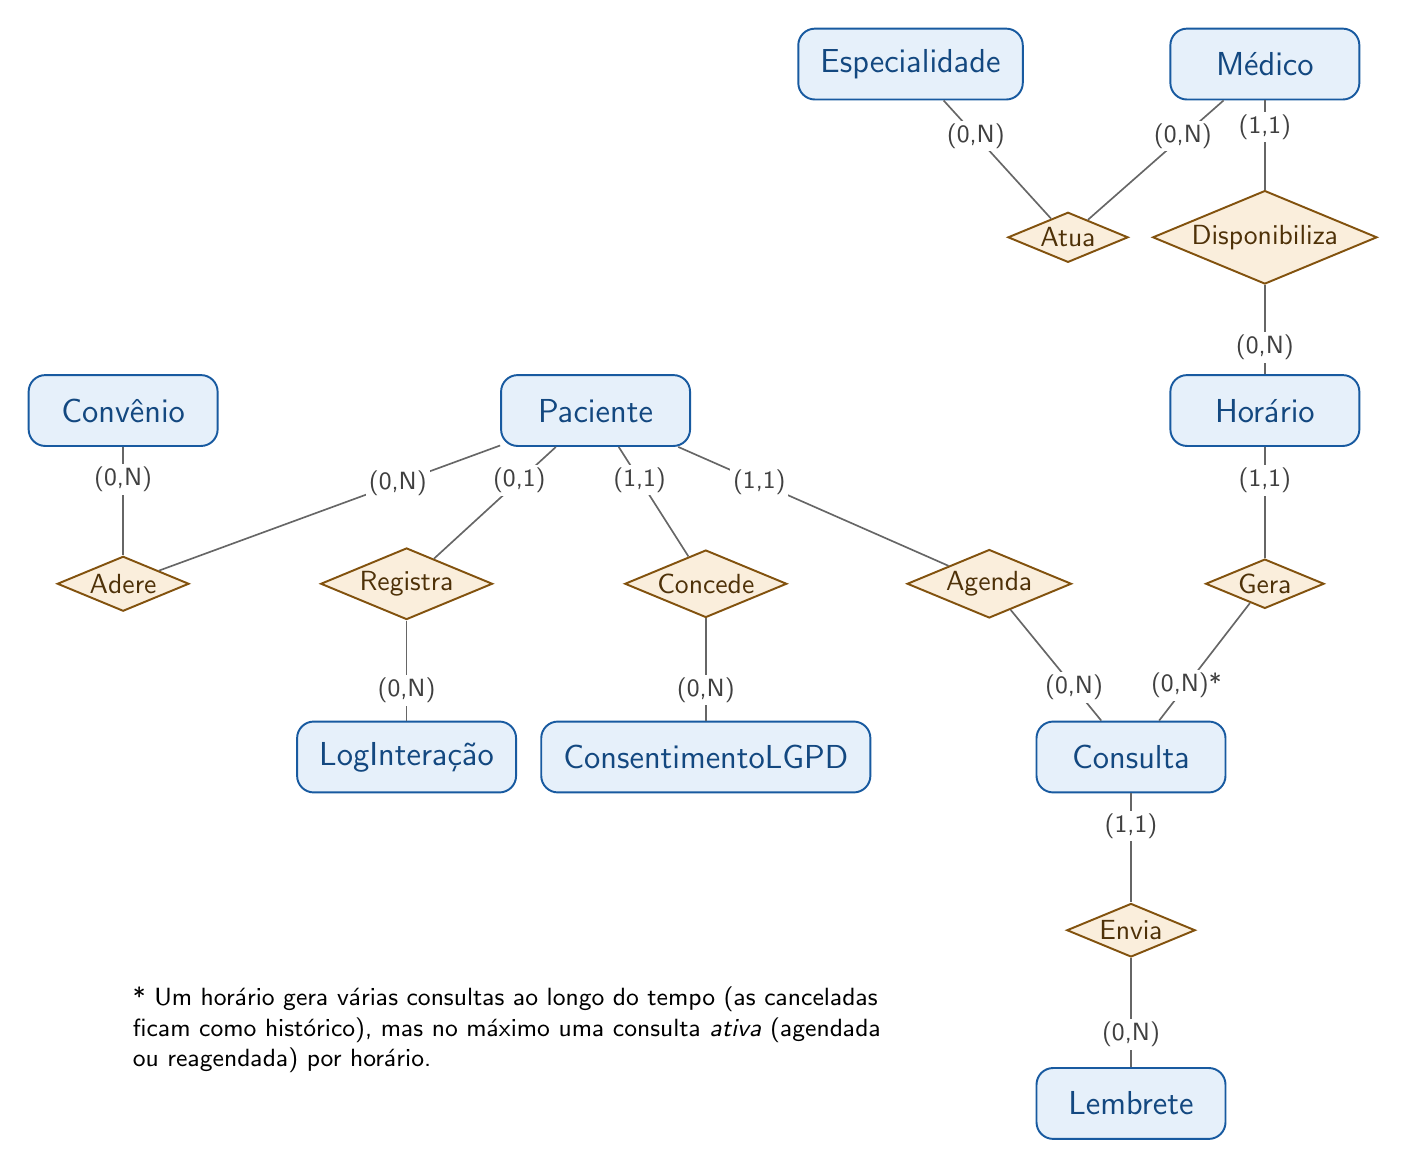
\begin{tikzpicture}
\node[ent] (esp)  at (10,0)    {Especialidade};
\node[ent] (med)  at (14.5,0)  {Médico};
\node[rel] (atua) at (12,-2.2) {Atua};
\node[rel] (disp) at (14.5,-2.2) {Disponibiliza};
\node[ent] (hor)  at (14.5,-4.4) {Horário};
\node[rel] (gera) at (14.5,-6.6) {Gera};

\node[ent] (conv) at (0,-4.4)  {Convênio};
\node[ent] (pac)  at (6,-4.4)  {Paciente};
\node[rel] (adere) at (0,-6.6)  {Adere};
\node[rel] (regi)  at (3.6,-6.6) {Registra};
\node[rel] (conc)  at (7.4,-6.6) {Concede};
\node[rel] (agen)  at (11,-6.6)  {Agenda};

\node[ent] (log)  at (3.6,-8.8) {LogInteração};
\node[ent] (cons) at (7.4,-8.8) {ConsentimentoLGPD};
\node[ent] (cta)  at (12.8,-8.8) {Consulta};
\node[rel] (envia) at (12.8,-11) {Envia};
\node[ent] (lem)  at (12.8,-13.2) {Lembrete};

\ligar{esp}{atua}{(0,N)}   \ligar{med}{atua}{(0,N)}
\ligar{med}{disp}{(1,1)}   \ligar{hor}{disp}{(0,N)}
\ligar{hor}{gera}{(1,1)}   \ligar{cta}{gera}{(0,N)*}
\ligar{conv}{adere}{(0,N)} \ligar{pac}{adere}{(0,N)}
\ligar{pac}{regi}{(0,1)}   \ligar{log}{regi}{(0,N)}
\ligar{pac}{conc}{(1,1)}   \ligar{cons}{conc}{(0,N)}
\ligar{pac}{agen}{(1,1)}   \ligar{cta}{agen}{(0,N)}
\ligar{cta}{envia}{(1,1)}  \ligar{lem}{envia}{(0,N)}

\node[font=\sffamily\small, text width=9.5cm, align=left, anchor=north west] at (0,-11.6)
  {* Um horário gera várias consultas ao longo do tempo (as canceladas ficam como histórico),
   mas no máximo uma consulta \emph{ativa} (agendada ou reagendada) por horário.};
\end{tikzpicture}
\end{document}
